% !TEX root = main.tex

%%%%%%%%%%%%%%%%%%%%%%%%%%%%%%%%%%%%%%%%%%%%%%%%%%%%%%%%%%%%%%%%%%%%%%%%%%%%%%%%%%%%%%%%%%%%%%%%
\section{結果}
%%%%%%%%%%%%%%%%%%%%%%%%%%%%%%%%%%%%%%%%%%%%%%%%%%%%%%%%%%%%%%%%%%%%%%%%%%%%%%%%%%%%%%%%%%%%%%%%

\subsection{実験課題1}
各周波数$f$における測定結果を以下の図4~図9に示す.
また,$\Delta x$は$10.0\,[\si{mm}]$に調整した.

\begin{figure}[H]
    \centering
    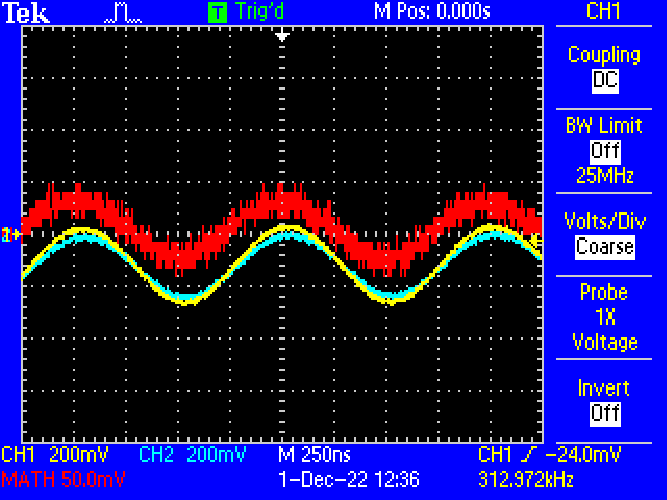
\includegraphics[scale=0.5]{F0001.pdf}
    \caption{$f=1\si{MHz}$のときの測定結果}
\end{figure}

\begin{figure}[H]
    \centering
    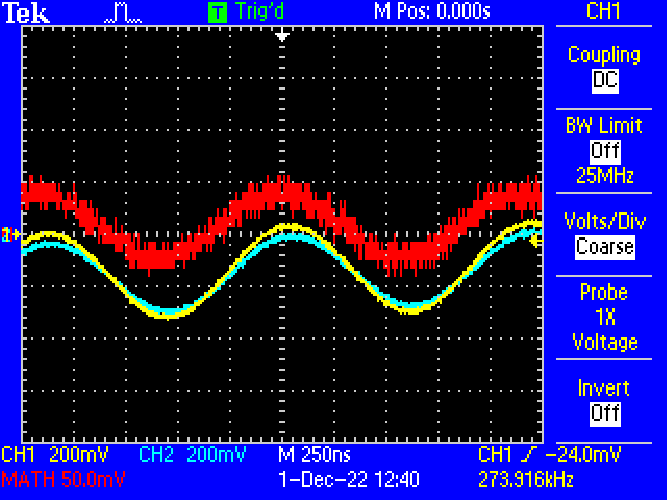
\includegraphics[scale=0.5]{F0002.pdf}
    \caption{$f=900\si{kHz}$のときの測定結果}
\end{figure}

\begin{figure}[H]
    \centering
    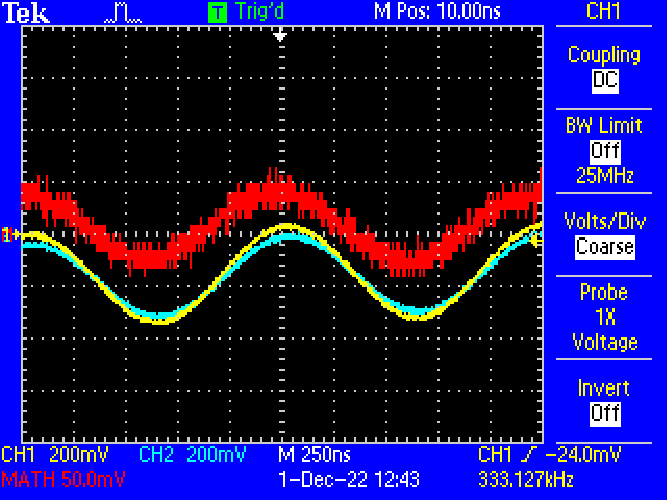
\includegraphics[scale=0.5]{F0003.pdf}
    \caption{$f=800\si{kHz}$のときの測定結果}
\end{figure}

\begin{figure}[H]
    \centering
    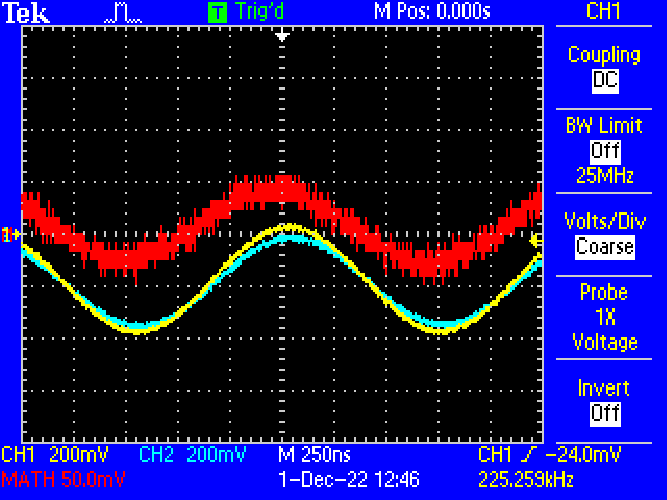
\includegraphics[scale=0.5]{F0004.pdf}
    \caption{$f=700\si{kHz}$のときの測定結果}
\end{figure}

\begin{figure}[H]
    \centering
    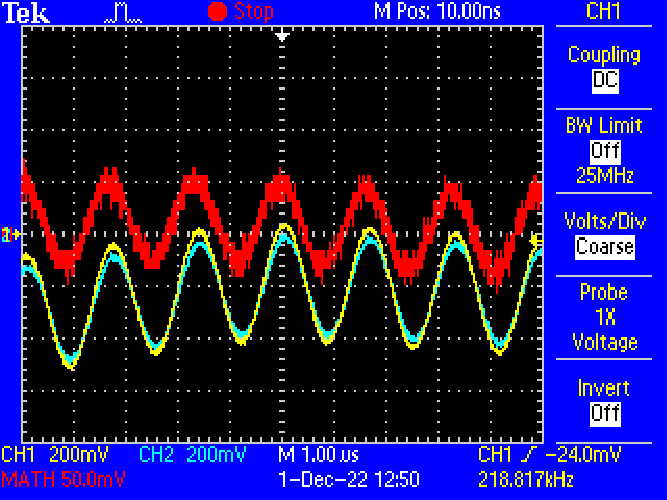
\includegraphics[scale=0.5]{F0005.pdf}
    \caption{$f=600\si{kHz}$のときの測定結果}
\end{figure}

\begin{figure}[H]
    \centering
    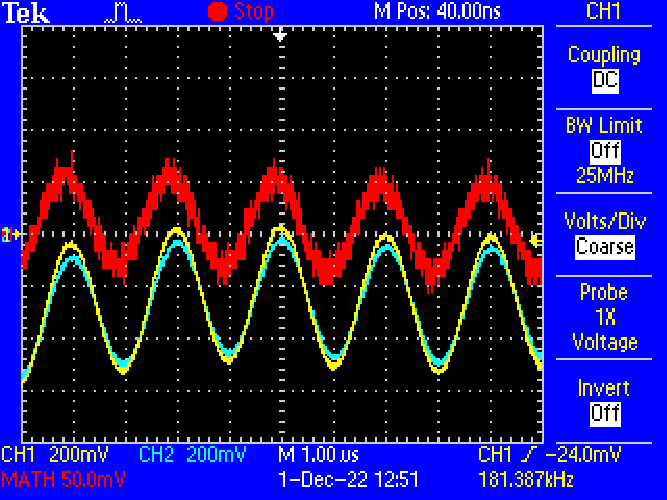
\includegraphics[scale=0.5]{F0006.pdf}
    \caption{$f=500\si{kHz}$のときの測定結果}
\end{figure}

\newpage

\subsection{実験課題2}
各周波数$f$における測定結果を以下の図10~図15に示す.


\begin{figure}[H]
    \centering
    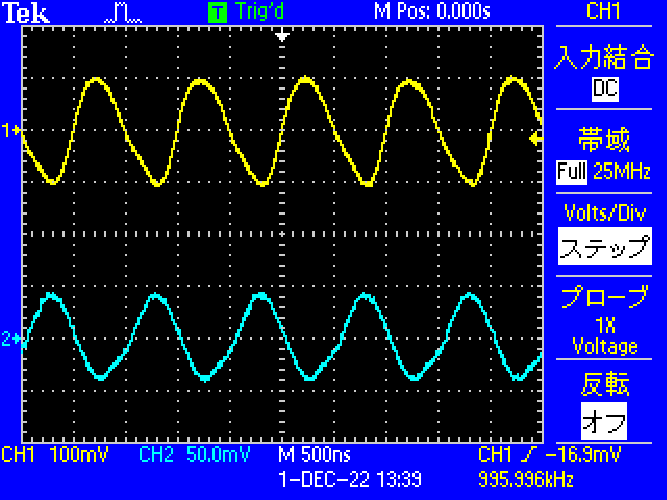
\includegraphics[scale=0.5]{TEK0001.pdf}
    \caption{$f=1\si{MHz}$のときの測定結果}
\end{figure}

\begin{figure}[H]
    \centering
    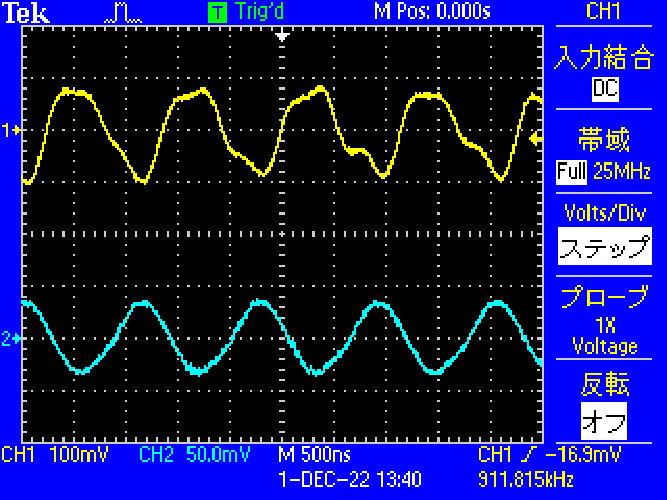
\includegraphics[scale=0.5]{TEK0002.pdf}
    \caption{$f=900\si{kHz}$のときの測定結果}
\end{figure}

\begin{figure}[H]
    \centering
    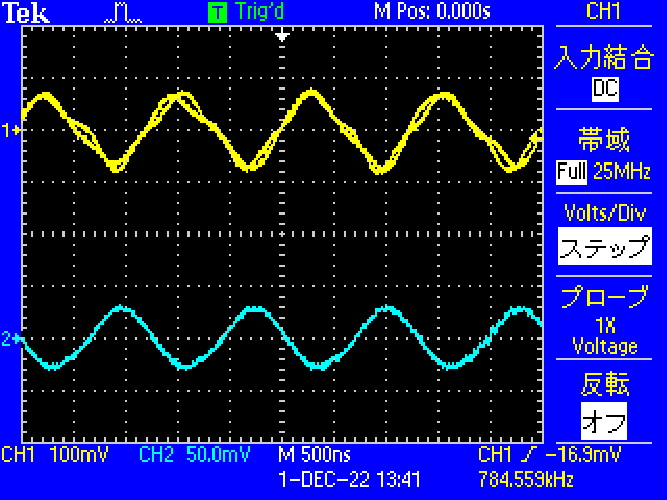
\includegraphics[scale=0.5]{TEK0003.pdf}
    \caption{$f=800\si{kHz}$のときの測定結果}
\end{figure}

\begin{figure}[H]
    \centering
    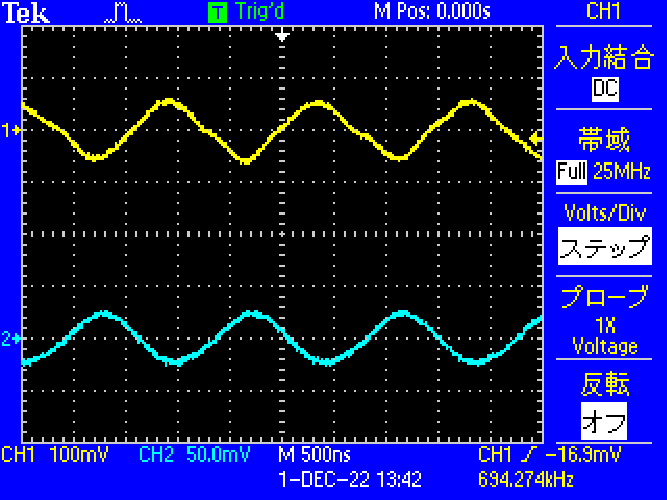
\includegraphics[scale=0.5]{TEK0004.pdf}
    \caption{$f=700\si{kHz}$のときの測定結果}
\end{figure}

\begin{figure}[H]
    \centering
    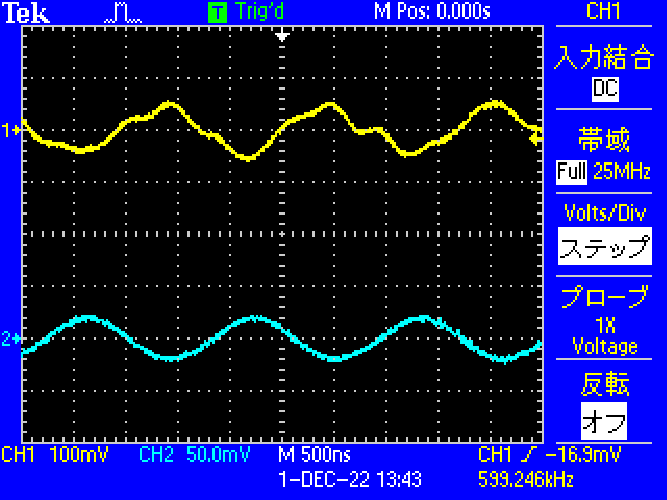
\includegraphics[scale=0.5]{TEK0005.pdf}
    \caption{$f=600\si{kHz}$のときの測定結果}
\end{figure}

\begin{figure}[H]
    \centering
    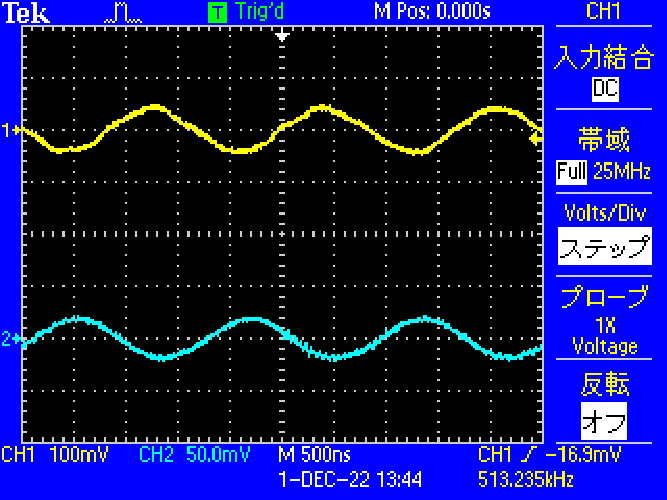
\includegraphics[scale=0.5]{TEK0006.pdf}
    \caption{$f=500\si{kHz}$のときの測定結果}
\end{figure}